
%!TEX root = ../thesis.tex
%*******************************************************************************
%****************************** Third Chapter **********************************
%*******************************************************************************
\chapter{Simulation Framework of SBND}
\label{ChapterSim}

% **************************** Define Graphics Path **************************
\ifpdf
    \graphicspath{{Chapter5/Figs/Raster/}{Chapter5/Figs/PDF/}{Chapter5/Figs/}}
\else
    \graphicspath{{Chapter5/Figs/Vector/}{Chapter5/Figs/}}
\fi

%********************************** %Opening  **************************************

%Modern physics experiments and MC
Many modern particle physics experiments heavily rely on simulations to study the physics capabilities of the detector, to develop physics analysis tools as well as to relate experimental data to an underlying theoretical model they attempt to probe.  
The most common technique in simulation is Monte Carlo (MC), by random sampling from probability density functions (PFDs).
PDFs can be modelled from theories, driven from experimental data or a combination of both.
Simulation is beneficial for an experiment like SBND in the early stage of development where the detector is not yet operational to record data.
The search for Heavy Neutral Leptons (HNLs) at SBND presented in this thesis employs simulated MC samples mimicking data.                                 
This enables an exploration of the detector physics capabilities in the regime of physics beyond the Standard Model.
%, given that the detector timing resolution can achieve nanosecond resolution.

The following chapter provides a detailed description of the simulation framework of SBND to output simulated products that ideally represent real data.
The chapter begins with an overview of the framework in Sec. \ref{sec:overview_sim}.
Following that, Sec. \ref{sec:gen_mevprtl} includes details of the generator employed to generate a signal event of HNLs and Sec. \ref{sec:gen_sm} provides the summary of the generators of SM neutrinos and cosmic muons.
Sec. \ref{sec:gen_response} covers the simulation of energy deposition as particles propagate through the detector and the detector response to the deposited energy.
Finally, some concluding remarks are provided in Sec. \ref{sec:sim_concluding_remarks}.

\newpage

%********************************** %First Section  **************************************
\section{Overview Of The Simulation Framework}
\label{sec:overview_sim}

Similar to many other LArTPCs, the software framework for simulation, reconstruction and analysis of SBND is provided by the LArSoft framework \cite{larsoft}. 
The framework was built for neutrino experiments sharing the same common feature of having LArTPCs, while still allowing for detector-specific customisation. 
This enables easy sharing of software tools across many collaborations including ArgoNeuT, MicroBooNE, ICARUS, SBND and DUNE. 
For example, the generator used to simulate HNLs, to be discussed in the next section, has been developed and shared across the SBND and ICARUS collaboration.

%Describe the overall workflow
The simulation framework of SBND under the LArSoft framework is depicted in Fig. \ref{fig:Sim_Workflow}.
The process begins with a generator to produce primary particles that enter the detector, as shown by the purple box.
The primary particles can be neutrinos, cosmic muons or BSM particles depending on the type of generator.
The propagation of the primary particle inside and outside the detector, and the resulting energy deposition is simulated using the Geant4 tool kit \cite{geant4}, as shown by the green boxes.
For interactions inside the detector, the charge and light yield are calculated from the energy deposition.
Ionisation electrons are propagated through the detector to the wire planes using the Wirecell tool kit \cite{wirecell}, as shown by the red boxes.
Scintillation photons are propagated to the photodetectors using a combination of a semi-analytical model and an optical library \cite{sbnd_pds_paper}, as shown by the blue boxes.
For interactions outside of the detector, only the energy depositions within CRT strips are converted into light yield, as shown by the orange box.
The detector response is then simulated for each detector subsystem.
By the end of this stage, the outputs from each detection subsystem ideally represent real data.

\begin{figure}[htbp!] 
\centering    
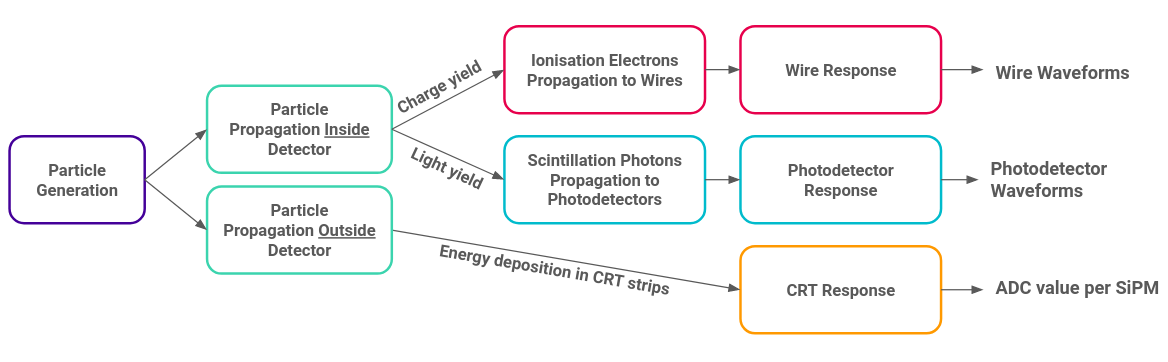
\includegraphics[width=1.0\textwidth]{Sim_Workflow}
\caption[Simulation Framework of SBND]{
Overview of the simulation framework of the SBND detector.
}
\label{fig:Sim_Workflow}
\end{figure}

\section{HNL Generator: MeVPrtl}
\label{sec:gen_mevprtl}

%MeVPrtl Workflow
BSM particles are generated using a generator called MeVPrtl, which was developed as a joint effort by collaborators from both ICARUS and SBND experiments.
There are several BSM models implemented in the MeVPrtl generator, including HNLs, Higgs portal scalars \cite{higgs_scalar} and heavy QCD axions \cite{qcd_axion}.
It is a modular generator, allowing for easy adaptations for different beam sources and detectors, as well as a direct interface with the existing LArSoft framework.
The workflow of the MeVPrtl is broken down into 4 stages, as illustrated in Fig. \ref{fig:MeVPrtl_Workflow}.
The generator begins with taking an input of meson fluxes, representing the particles produced from a beam source.
It then simulates the meson decaying to a BSM particle.
The BSM particle is propagated to the detector and decays back into SM observables.

\begin{figure}[htbp!] 
\centering    
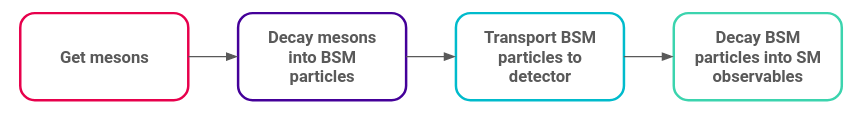
\includegraphics[width=1.0\textwidth]{MeVPrtl_Workflow}
\caption[MeVPrtl Generator Workflow]{
Overview of the workflow of the MeVPrtl generator.
}
\label{fig:MeVPrtl_Workflow}
\end{figure}

%Each stage validation
For generating HNLs coming from the BNB, the generator begins with sampling the $K^{+}$ fluxes of the BNB (See Fig. \ref{fig:BNB_Meson_Flux}, Sec. \ref{sec4BNB}).
Instead of decaying into SM neutrinos, the kaons decay into HNLs, with the branching ratio defined by Eq. \ref{eq:kaon_decay_hnl} (See Sec. \ref{sec2Production}).
The daughter HNL and lepton are simulated using the two-body decay at rest in the centre of mass frame of the parent kaon and then boosted to the parent's lab frame by Lorentz boost.
Due to HNLs having mass, HNLs have less transverse momentum than SM neutrinos and therefore are more collimated, travelling preferably to the parent kaon direction.
The Lorentz boost can flip the directions of HNLs that are emitted backwards, originating from low energy kaons \cite{DavidePhD}.
HNLs are propagated to the detector by the ray tracing method, which forces HNLs to hit the SBND detector by picking a direction that impinges the particles at the detector's front face.  
The probability of enforcing the detector intersection is also computed.

Example angular distributions in the lab frame of parent kaons and HNLs that arrive at the SBND detector are shown in Fig. \ref{fig:kaon_hnl_angle2beam}.
Fig. \ref{fig:kaon_angle2beam} shows the angle to the beam direction of 7 different kaon parents having energies peaking at approximately $0.5\sim1$ GeV, each of a different colour dashed line.
The resulting HNL of mass 240 MeV from each kaon is shown in Fig. \ref{fig:hnl_angle2beam}, in the same colour dashed line as the parent kaon.
Here, it can be seen that the angles to the beam direction of HNLs are very small as all the lines overlap within $ < 5^\circ$.
This demonstrates that the acceptance angle of the HNLs to hit the SBND detector is very collimated, such that only very forward-going HNLs are most likely to intersect the detector.

\begin{figure}[htbp!]
        \centering
        \begin{subfigure}[b]{0.495\textwidth}
            \centering
            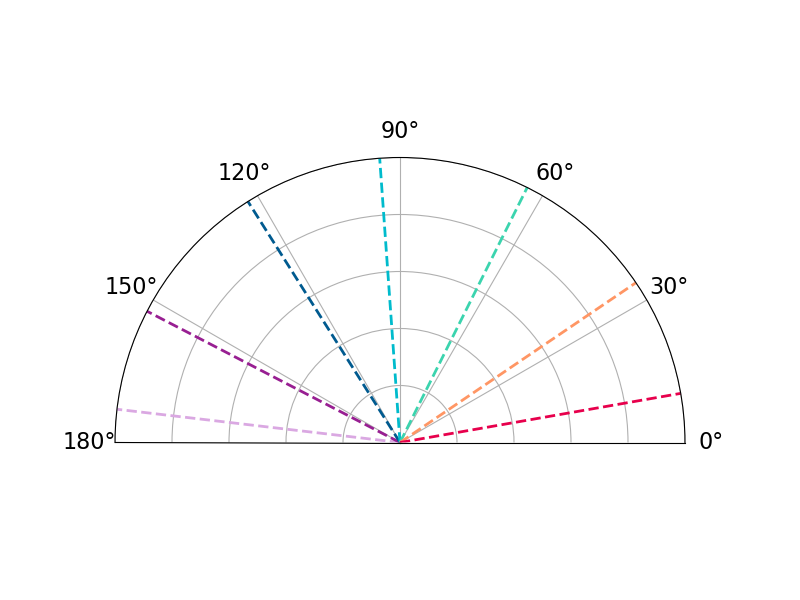
\includegraphics[width=\textwidth]{kaon_angle}
            \caption{Kaons}%
            \label{fig:kaon_angle2beam}
        \end{subfigure}
        \hfill
        \begin{subfigure}[b]{0.495\textwidth}  
            \centering 
            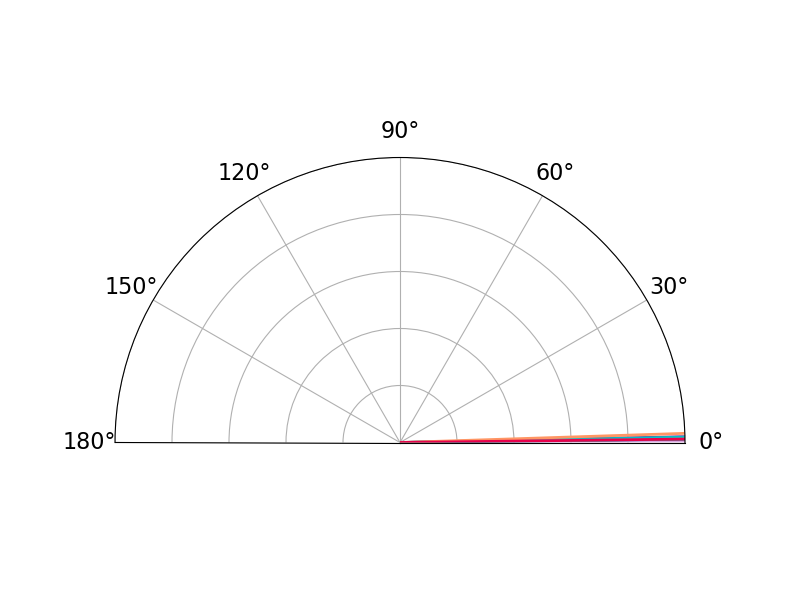
\includegraphics[width=\textwidth]{hnl_angle}
            \caption{HNLs}%
            \label{fig:hnl_angle2beam}
        \end{subfigure}
        \caption[Angle To The Beam Direction of Kaons and Resulting HNLs Polar Plots]{
	Polar plots showing the angle to the beam direction of 7 different parent kaons (left) and of the resulting HNLs that arrive at the detector (right).
	}
        \label{fig:kaon_hnl_angle2beam}
\end{figure}

The resulting fluxes of HNLs arriving at the SBND detector are depicted in Fig. \ref{fig:HNL_Energy_Spectrum} for the mass range between 140 and 260 MeV.
The fluxes plotted here, and all subsequent kinematics plots in this section, are labelled \textit{true}, indicating they are at the truth level and not yet passed through detector simulation and reconstruction.
The fluxes are normalised to the same mixing $|U_{\mu4}|^{2} = 1 \times 10^{-7}$ and an exposure of $1 \times 10^{21}$ POT projected for 3 years of data taking.
At the same mixing, the expected HNL rate decreases with lower mass since the branching ratio of $N \rightarrow \nu\pi^0$ decreases with lower mass (See Fig. \ref{fig:branchingRatio} Sec. \ref{sec2Decay}).
Additionally, given that the $K^{+}$ flux peaks around 0.5 GeV and decreases at higher energy (See Fig. \ref{fig:BNB_Meson_Flux}, Sec. \ref{sec4BNB}), the HNL fluxes also mainly concentrate in the low energy region, and substantially decrease at higher energy. 
Moreover, across the HNL mass range, there are more energetic HNLs at a lower mass than at a higher mass.
This is due to HNLs coming from a kaon decay and therefore, the lighter the HNL mass, the more kinetic energy is available.
Finally, all the HNL fluxes have a sharp peak near zero, corresponding to HNLs resulting from Kaons Decay At Rest (KDAR).

Upon their arrival at the detector, HNLs decay back into the SM observables.
For the $\nu\pi^{0}$ final state, the width of the decay is defined by Eq. \ref{eq:pi0} (See Sec. \ref{sec2Decay}).
The kinematics of the decay products are simulated for HNLs isotropically decay in the rest frame and then boosted to the lab frame by Lorentz boost.
Since the parent HNL is very forward-going, the daughter $\pi^0$ is also forward-going, with momenta dependency on the mass of the parent HNL. 
Fig \ref{fig:pi0_distribution} shows the true energy and angle to the beam distributions for the daughter $\pi^0$.
The plots are area-normalised for comparison across the mass range of the parent HNL from 140 to 260 MeV. 
The peak in the energy distribution at low energy and the peak in the angular distribution at high angle are from the $\pi^0$ coming from low energy HNLs from KDAR.
The energy distribution of the $\pi^0$ decreases as the HNL mass increases since heavier HNLs are less energetic and therefore, less energy is available for the $\pi^0$.
As a result, the angle to the beam of the $\pi^0$ also widens with heavier HNLs.
However, at the heaviest HNL mass of 260 MeV considered in the search, the $\pi^0$ is still very collimated since its angular distribution concentrates in the region $< 30^\circ$. 
Therefore, the di-photon showers from the HNL-originated $\pi^0$ are expected to be more forward-going than those originating from SM neutrinos.

\begin{figure}[t!] 
\centering    
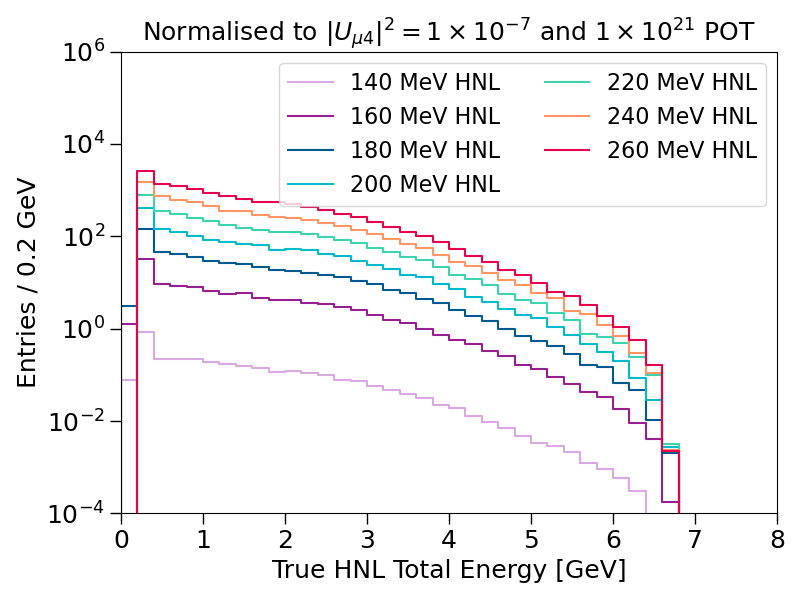
\includegraphics[width=0.5\textwidth]{HNL_Energy_Spectrum}
\caption[Simulated HNL Fluxes at the Front Face of SBND]{
Simulated HNL fluxes at the front face of SBND.
}
\label{fig:HNL_Energy_Spectrum}

%\end{figure}
%\begin{figure}[bp!]
\vspace{0.5cm}
        \centering
        \begin{subfigure}[b]{0.495\textwidth}
            \centering
            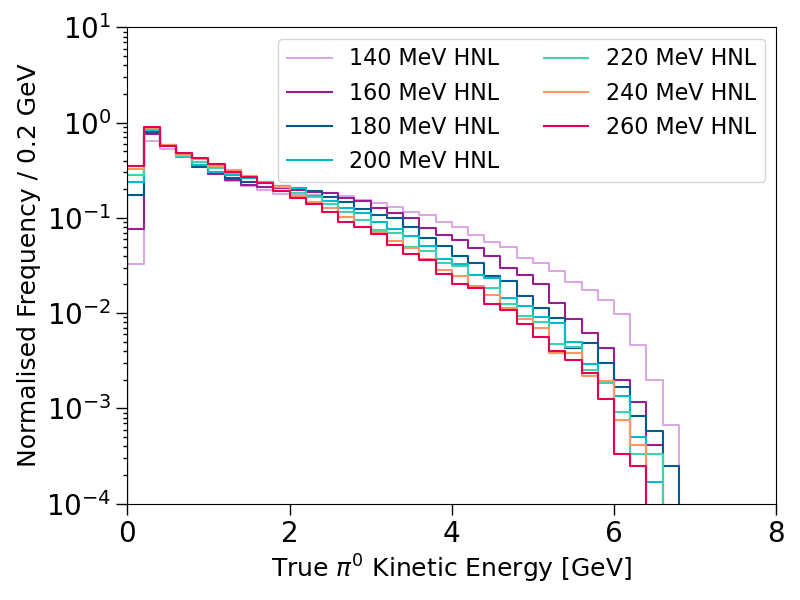
\includegraphics[width=\textwidth]{pi0_energy}
            \caption{Energy Distribution}%
            %\label{fig:kaon_angle2beam}
        \end{subfigure}
        \hfill
        \begin{subfigure}[b]{0.495\textwidth}  
            \centering 
            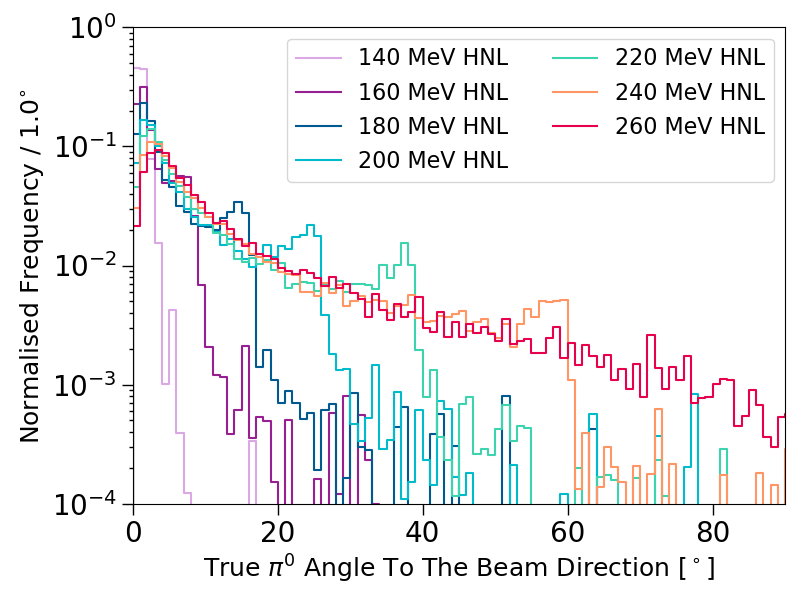
\includegraphics[width=\textwidth]{pi0_angle2Beam}
            \caption{Angle to the Beam Direction Distribution}%
            %\label{fig:hnl_angle2beam}
        \end{subfigure}
        \caption[Kinematics Distributions of Neutral Pions From HNLs]{Kinematics distributions of $\pi^0$ from HNLs decaying inside SBND.}
        \label{fig:pi0_distribution}
\end{figure}

The timing delay between HNLs compared to SM neutrinos due to HNLs being more massive provides an advantageous edge in the search for HNLs at SBND. 
The components that make up the time of flight for an HNL or a SM neutrino produced from the BNB and propagating to the SBND detector are illustrated in Fig. \ref{fig:tof_beam_to_detector}.
The first component is the spill time of the protons from the Booster synchrotron, $t_{spill}$, as shown by the red arrow.
The structure of $t_{spill}$ is the beam bucket structure made up of 81 Gaussian buckets with a width of 1.308 ns and a spacing of 19 ns, which is the same for both HNLs and SM neutrinos.
Details of the beam structure were previously detailed in Sec. \ref{sec4BNB}.   

The second component is the time of the secondary mesons, $t_{meson}$, as shown by the blue arrow.
This is the period from when the mesons are produced until they decay into HNLs or SM neutrinos.
This time accounts for the duration that the mesons travel down the decay pipe, and might interact, re-scatter or decay into other mesons.
In the case of HNLs, $t_{meson}$ is primarily the time of flight of the charged kaon $K^+$ before decaying into an HNL.
On the other hand, SM neutrinos come from a variety of parent mesons $t_{meson}$. % (See Fig. \ref{fig:BNB_neutrino_flux}).
In both cases, $t_{meson}$ introduces some smearing to the nanosecond-bucket structure of $t_{spill}$.

The last component is the time of flight of the SM neutrino or the HNL from the creation point to the interaction point inside the SBND detector.
In the case of SM neutrinos, since they are nearly massless, their velocity can be approximated as the speed of light. 
Then, the time of flight of the SM neutrino is  
\begin{equation}
	t_{\nu} = \frac{d_{\nu}}{c}
\end{equation}
where $d_{\nu}$ is the distance of a neutrino from the creation point to the interaction point inside the detector.
Meanwhile, HNLs are massive and therefore, travel at a velocity $v_N < c$.
The time of flight of the HNL is
\begin{equation}
	t_{N} = \frac{d_{N}}{v_N}
\end{equation}
where $d_N$ is the distance of a HNL from the creation point to the decay point inside the detector.
Additionally, since the energy of the HNL decreases with its mass, the heavier it is, the slower its velocity.
Thus, heavier HNLs arrive even later compared to lighter HNLs.

\begin{figure}[hb!] 
\centering    
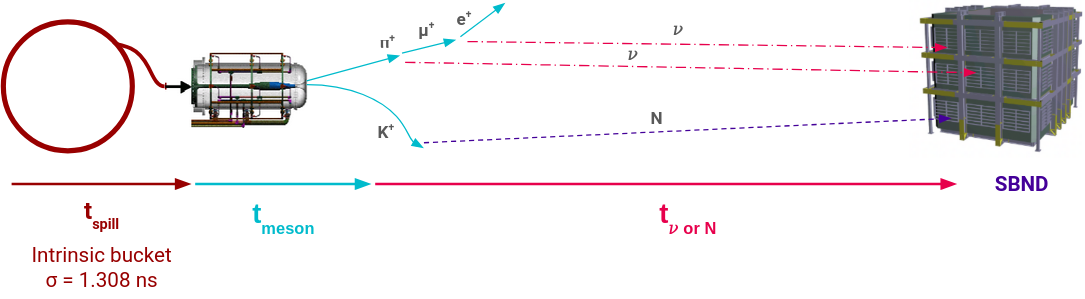
\includegraphics[width=1.0\textwidth]{tof_beam_to_detector}
\caption[Time of Flight of Particles From the BNB to SBND Diagram]{
Diagram depicting the time of flight of a particle from its production in the BNB to its detection in the SBND detector.
}
\label{fig:tof_beam_to_detector}
\end{figure}

The advantage of the MeVPrtl generator is the consistency of simulating the time of flight of HNLs to the GENIE generator for simulating SM neutrinos.
Fig. \ref{fig:full_beam} shows the true simulated arrival time of SM neutrinos, in the dashed grey line, and 260 MeV HNLs, in the solid red line, at the front face of the SBND detector, recovering the beam spill structure of the BNB.
The plot is area-normalised to enable the comparison between the two particles. 
Since SM neutrinos travel nearly at the speed of light, less smearing is introduced and the timing distribution shows sharp Gaussian peaks.
On the other hand, HNLs travel slower and add additional smearing and delay tails to the Gaussian peaks.
For clarity, shown in Fig. \ref{fig:beam_modulus}, is the result of 81 Gaussian peaks overlaid into 1 peak by taking the modulus of 19 ns.
The timing distribution of the HNLs shows a clear difference from that of SM neutrinos, where delay tails on either side of the Gaussian peak can be seen.
Between the mass of 140 to 260 MeV, the delay tails however do not increase significantly with mass.

\begin{figure}[ht!] 
\centering    
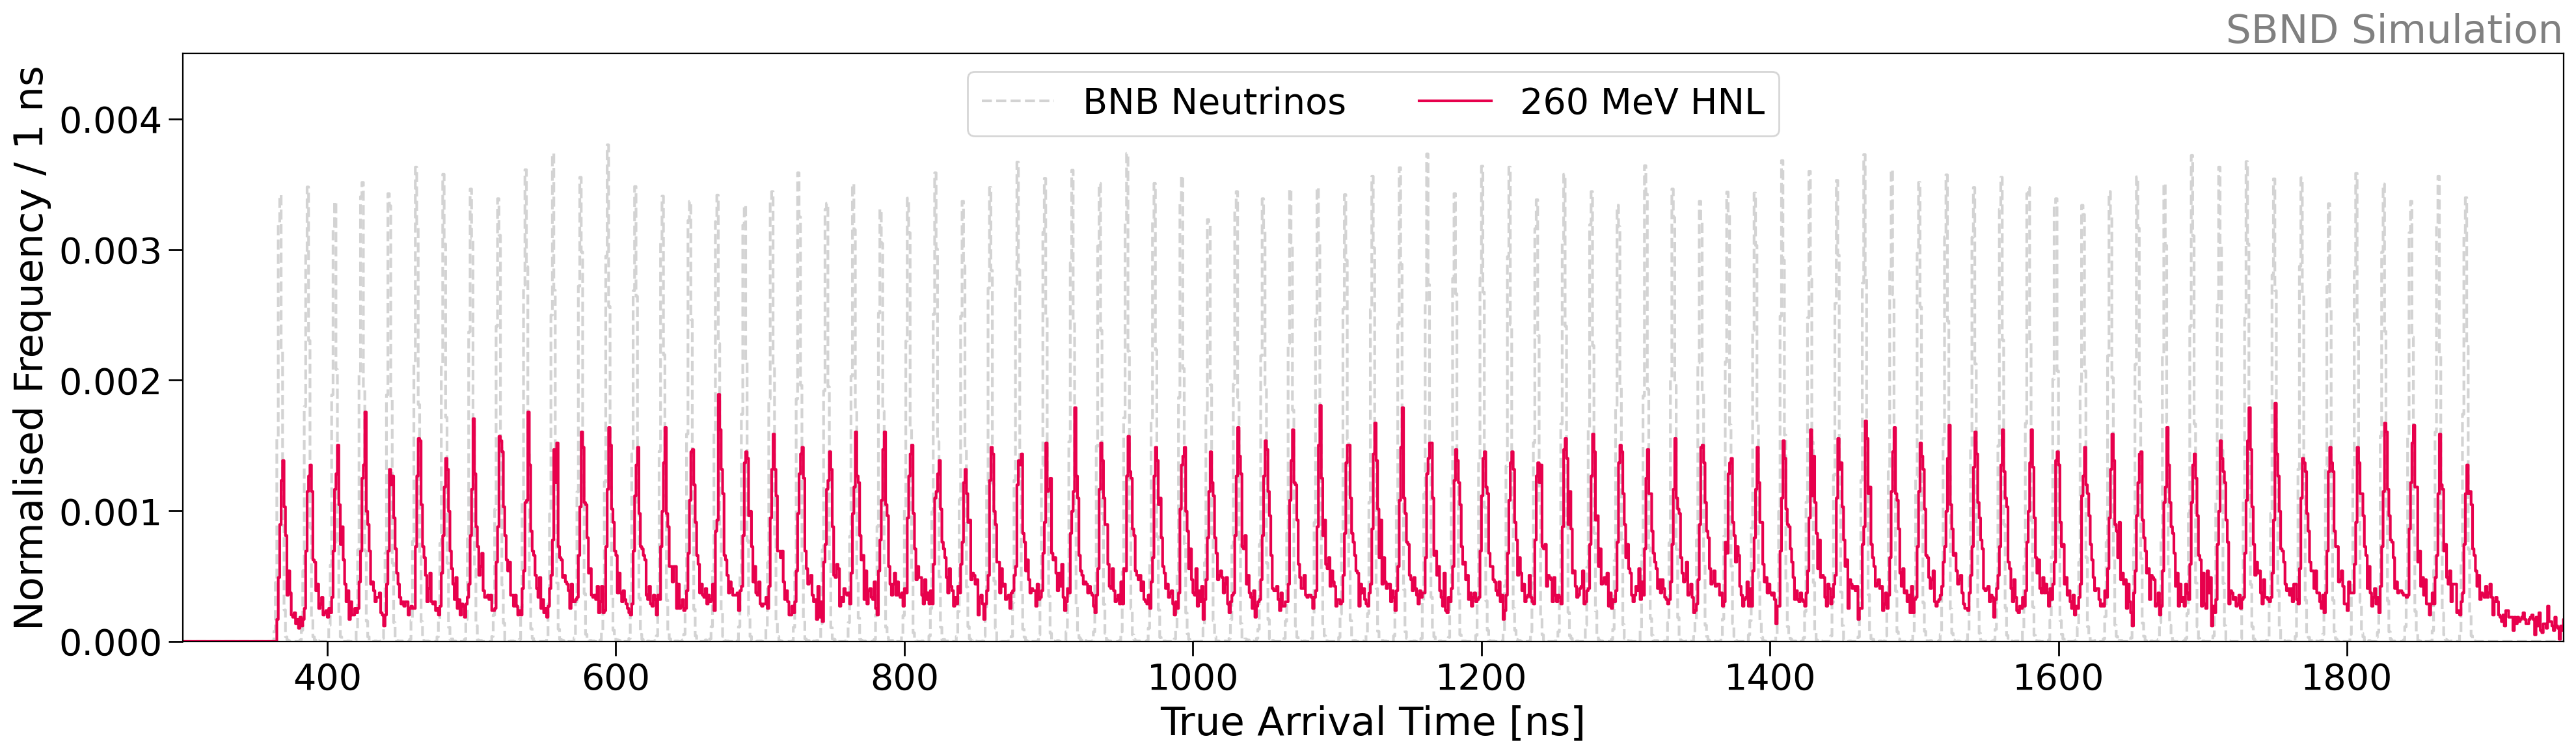
\includegraphics[width=1.0\textwidth]{full_beam}
\caption[Arrival Time of SM Neutrinos and HNLs at the Front Face of SBND]{
Arrival time distribution at the front face of the SBND detector for SM neutrinos and HNLs. 
}
\label{fig:full_beam}
%\end{figure}
%\begin{figure}[htbp!] 
\vspace{0.5cm}
\centering    
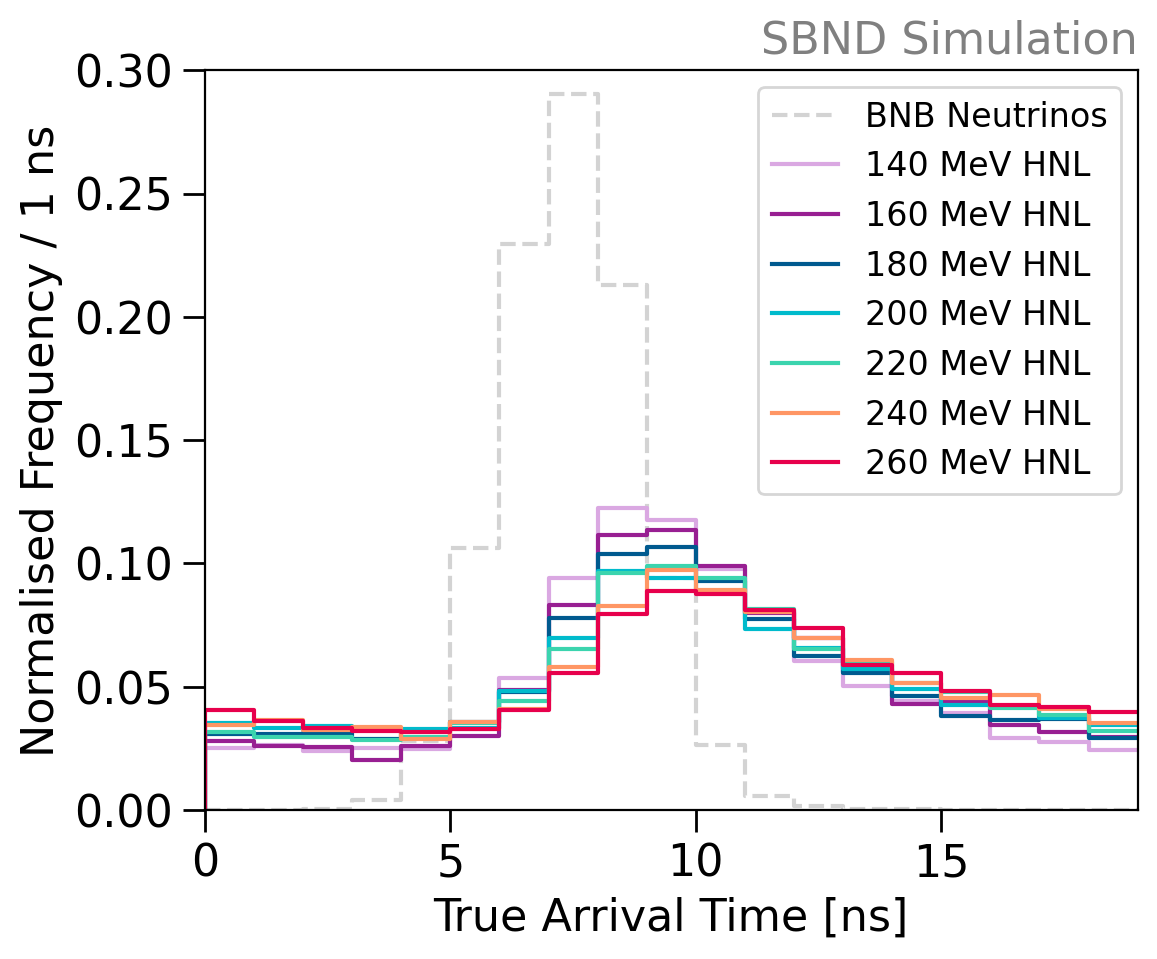
\includegraphics[width=0.495\textwidth]{beam_modulus}
\caption[Modulus of the Arrival Time Distibutions of SM Neutrinos and HNLs]{
Modulus of the arrival time distribution for SM neutrinos and HNLs. 
}
\label{fig:beam_modulus}
\end{figure}

\newpage
\section{SM Generators}
\label{sec:gen_sm}

For generating backgrounds from SM neutrinos and cosmic muons, the two generators are GENIE \cite{genie} and CORSIKA \cite{corsika} respectively.
Each generator will be discussed in Sec. \ref{sec:gen_genie} and Sec. \ref{sec:gen_corsika}.

\subsection{Neutrino Generator: GENIE}
\label{sec:gen_genie}

%Overview of GENIE
SM neutrino interactions are generated by the GENIE generator \cite{genie}, which provides a selection of theoretical and empirical models for different physical processes.
These models can be combined into a \textit{tune}, which is a set of optimised parameters used in the simulation for a better agreement between model and data.
The GENIE tunes are made using an extensive dataset of electron, neutrino and hadron scattering experiments.
The SBND collaboration is planning to use a tune that was specifically developed to serve as a baseline model for the SBN and DUNE oscillation analysis.
Details for the basis of the tune can be found in Table 1 in Ref. \cite{genie_tune}, with ongoing developments on the choice of models documented in Ref. \cite{genie_tune_github}.  

%What kind of tune are being used
In general, GENIE first selects a nuclear model that describes the momenta and potential energy of the nucleon to model nuclear effects.                                                    
Then, the neutrino flux and the integrated cross section model are used to compute the probability that a neutrino interaction occurs.
The differential cross section is then used to determine the type of neutrino interaction and the kinematic range.
The neutrino interaction types include quasi-elastic, resonant, coherent, deep inelastic and $\nu$-e elastic scatterings.
In addition, neutrino interacting with an argon nucleus can produce hadrons within the nucleus.
The hadrons propagate through the nucleus, interacting via different modes such as charge exchange, elastic scattering, absorption and pion production.
Consequently, the hadron-nucleus interaction modifies the final state particles and their kinematics.
Thus, the hadron transport interaction model is crucially important for predicting the final observables of neutrino interactions.

In addition to the tune, GENIE also provides a re-weighting scheme to evaluate the systematic uncertainties for a model chosen in the tune.
Due to the scarcity of neutrino interaction data, particularly for $\nu-Ar$ interactions, the uncertainties in cross section modelling tend to be very large. 
The neutrino interaction re-weighting scheme and the resulting systematics uncertainties impact the HNL search will be discussed in detail in Sec. \ref{sec:bkg_error}.

At SBND, GENIE simulates neutrino interactions occurring both inside and outside of the detector volume, with a boundary defined in Fig. \ref{fig:Rockbox_Volume}.  
All interactions occurring inside the detector volume are strictly kept, as shown by the dark blue box.
Outside of the detector, a buffer volume is defined as 5 m surrounding the detector volume, as shown by the light blue box.                       
An additional Rockbox volume is defined by extending the buffer volume backwards in the beam direction ($z$-axis) up to 15 m in front of the buffer volume, as shown by the orange box.
Both these volumes are referred to together as the \textit{Rockbox} volume in this thesis.
Neutrino interactions within this volume are kept because their products can potentially deposit energy in the detector.
These interactions are referred to as \textit{dirt} neutrinos and constitute a significant background to the HNL search.
The background rejection of dirt neutrinos will be covered in Chapter \ref{ChapterSelect}.

\begin{figure}[htbp!] 
\centering    
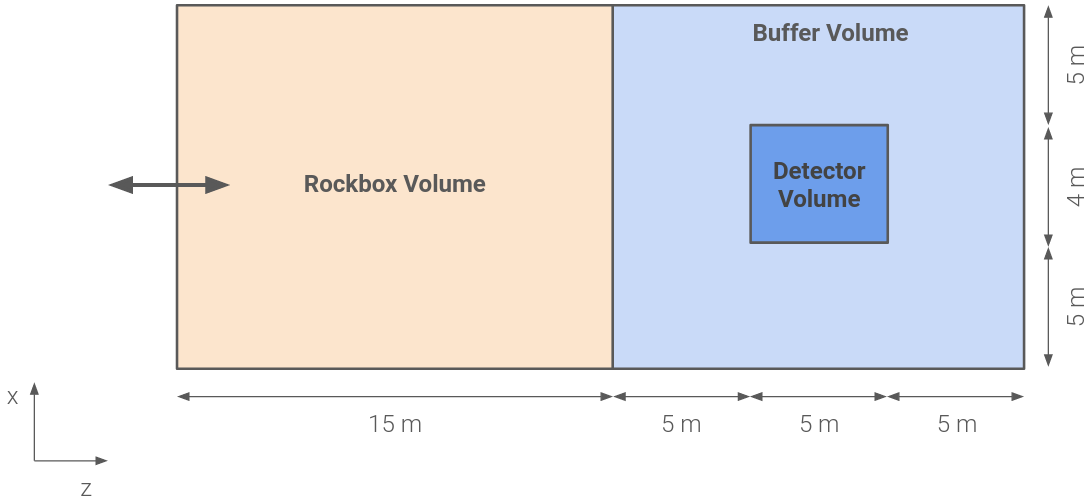
\includegraphics[width=0.85\textwidth]{Rockbox_Volume}
\caption[Volume Boundary of The GENIE Generator]{
Volume boundary defined by the GENIE generator to simulate neutrino interactions occurring inside and outside of the detector volume. 
}
\label{fig:Rockbox_Volume}
\end{figure}

\subsection{Cosmic Generator: CORSIKA}
\label{sec:gen_corsika}

Cosmic interactions are simulated using the CORSIKA generator \cite{corsika}.
The generation begins with producing high energy primary particles incident in the Earth's atmosphere, of which only primary protons are kept. 
The primaries are then propagated through the atmosphere, interacting with the air to produce secondary decays until reaching the Earth's surface.
Within the SBND simulation geometry, this surface is specified to be just above the roof of the detector building.
The surviving particles are then propagated to the SBND detector.

%Why cosmic simulation is important
From a triggering perspective, there are two types of comic muons as follows 
\begin{coloritemize}
        \item\textbf{In-time} cosmic muons cross the detector at the same time as SM neutrinos being present inside the detector, such that the muons are \textit{inside} the beam spill window. The cosmic muons produce enough light to induce a beam trigger.                            
        \item\textbf{Out-of-time} cosmic muons occur regardless of the trigger conditions. The muons cross the detector \textit{outside} the beam spill window but within the readout window.  
\end{coloritemize}
However, at the time of writing, triggering simulation is currently a work in progress at SBND and there not being simulated in the workflow. 
Only the timing requirement is simulated to keep only cosmic muons occurring within the readout window.
The simulation currently does not accurately reflect the cosmic rate once factoring triggering conditions and therefore, comparison to data is necessary. 

Being a surface-level detector, it is vitally important to understand the cosmic background at SBND due to the exposure to a high cosmic rate.
Once SBND is operational, a particularly useful measurement is the rate of cosmic muons that cause a beam trigger, however, in the absence of the beam.
This is equivalent to measuring the rate of cosmic muons that produce sufficient energy inside the detector to mimic SM neutrino interactions.
This measurement allows for validation against the CORSIKA generator sampling of the cosmic topology and kinematic distribution. 
Moreover, it also provides an expected cosmic rate given a triggering condition, which can be subsequently added to the simulation framework to better constrain the cosmic background.                

\section{Particle Propagation and Detector Response Simulation}
\label{sec:gen_response}


After the generation stage of the simulation workflow, simulated particles are propagated through the detector and deposit energy, producing ionisation electrons and scintillation photons.
The detector response to the ionisation electrons and scintillation photons is subsequently simulated, mimicking data. 
Sec. \ref{sec:gen_g4} first covers the simulation of particle propagation and energy deposition.
Following that, Sec. \ref{sec:wire_response}, \ref{sec:pds_response} and \ref{sec:crt_response} provides a description of the simulation of the TPC, PDS and CRT response. 

\subsection{Particle Propagation Simulation}
\label{sec:gen_g4}

Once a particle is simulated inside the detector, it is propagated through the detector using the Geant4 tool kit \cite{geant4}.
Geant4 propagates the particle by each step $dx$, where the step length is randomised and capped at 0.3 mm (one order of magnitude less than the wire pitch).
At each step, physics processes are applied to the particle, such as energy deposition, interaction, decay and so on.
The step propagation also accounts for the electric field distortion caused by the space charge effect due to high exposure to cosmic muons.
%For example of the $\nu\pi^0$ final state of HNLs, the $\nu$ escapes the detector without interacting while the $\pi^0$ is simulated to decay into a di-photon shower by Geant4.
%Then, Geant4 simulates the energy deposition of the resulting di-photon shower.

The main physics process for energy deposition in the detector is ionisation by charged particles.
Similarly to the theory detailed in Sec. \ref{sec3:creation}, the Geant4 tool kit simulates the ionisation process following the Bethe-Bloch formalism tuned to data \cite{geant4_ions}.
The number of ionisation electrons and scintillation photons from the deposited energy is computed using the ModBox recombination model with ArgoNeuT parameters \cite{argoneut_recomb}, and the charge-light anti-correlation from Eq. \ref{eq:Q} and \ref{eq:L}. 
Further discussion about the simulation of recombination, and the impacts of delta ray fluctuations on recombination will be detailed in the forthcoming Sec. \ref{sec7:delta}.
The result from the Geant4 tool kit is a complete set of charge and light yields along the primary particle trajectories through the detector and the hierarchy of the daughter particles produced from the primary.

\subsection{Wire Response Simulation}
\label{sec:wire_response}

Ionisation electrons are simulated to drift towards the wire planes using the WireCell tool kit \cite{wirecell}.
The simulation transports the electrons and introduces smearing due to detector effects for transporting electrons through liquid argon under an electric field, which is previously discussed in Sec. \ref{sec:edrift}.
This includes charge attenuation due to impurities, longitudinal and transverse diffusion and finally space charge effect.

Once drifting electrons arrive at the wire planes, a convolution of the field response and the electronic response is performed.                                                                                                          
The field response describes the current induced on wires due to ionisation electrons drifting past the induction planes.                                                                                                           
The electronic response describes the amplification and shaping of each wire's induced current by pre-amplifiers.
The response functions are in two dimensions, time versus wire.
This is to account for the long range charge induction effect on wire signal shapes.
A digitisation step is then applied to produce an ADC-level, time-domain waveform for each wire channel.
The waveform is parameterised by the ADC resolution, voltage range and baseline specification of the wire readouts.
Finally, inherent electronic noise is added to the waveform to better match to observed data.
MC waveforms at this stage ideally represent real data waveforms recorded by the wire readouts.

\subsection{Photon Detection System Response Simulation}
\label{sec:pds_response}

Scintillation photons are simulated to propagate to optical detectors, accounting for transport effects previously detailed in Sec. \ref{sec:photonprop} such as Rayleigh scattering and boundary effects.
In-depth details of the light simulation can be found in Ref. \cite{sbnd_pds_paper}.
The simulation uses a combination of a semi-analytical model described in Ref. \cite{pds_sim}, and an optical library model available in LArSoft.
The choice of which model to use depends on the location of the photon production.
The semi-analytical model is used for those produced inside the active volume of the SBND detector, whilst the optical library model is used for those that originate outside of this volume.

The semi-analytical model calculates on-the-flight the geometrical aperture for each optical detector to a scintillation point, given that the emission of scintillation photons is isotropic.
The model also extends to both direct visible photons and also reflected VUV photons. 
Corrections for photon transport effects are applied to the number of photons detected by an optical detector.
However, the semi-analytical method is limited by the geometrical information and does not include scintillation outside of the detector volume, for example, cosmic muons crossing behind an optical detector can produce non-negligible photons.
Since PMTs are the primary subsystems for triggering, it is vital to consider this second-order contribution of photons for triggering studies.
The optical library stores information on the fraction of incident photons for each optical detector for a given scintillation location, which can be looked up for any detector-location pairs during 
simulation. 

For each type of optical detector, PMTs and X-ARAPUCAs, a respective photon detection efficiency is applied to the number of detected photons.
Signal amplification and digitization are simulated, converting photons into an output signal known as a single electron response.
Then, signal shaping such as overshoot and undershoot due to the AC circuit of the optical detectors are applied.
Finally, random fluctuation in the signal integral and non-linearity response at high light intensities are applied to better mimic data.
The final output is MC optical waveforms for each type of optical detector, ideally the same as data. 

\subsection{Cosmic Ray Tagger Response Simulation}
\label{sec:crt_response}

The energy deposition outside of the cryostat from the Geant4 simulation stage in Sec. \ref{sec:gen_g4} is considered if it crosses CRT strips.
It is converted into photons within a strip and propagated down optical fibres towards the SiPMs for detection.
The collection efficiency per SiPM is accounted for by dividing the light yield between the fibres on either side of the strip, based on the lateral position of the energy deposition within the strip.
Propagation effects and signal attenuation are also simulated.
Finally, the electronic response is simulated for the CRT readout, by assessing if a pair of SiPMs within a strip goes above a threshold within a pre-defined coincidence window.
To better mimic the readout electronics of CRTs that process 32 SiPMs at a time, MC outputs of CRTs are in a group of 32 ADC values, where each value corresponds to a SiPM.

\section{Concluding Remarks}
\label{sec:sim_concluding_remarks}

The simulation framework of SBND described here shares the same purpose as with many other modern particle physics experiments, to help understand and improve the detector performance and physics capabilities.
This is done by simulating the end-to-end process from when a particle is produced, to how it deposits energy inside the detector and consequently, the detector response to the energy deposition.
The MC output of the simulation ideally mimics data, providing the foundation to perform different types of exploratory studies before SBND becomes operational.
For example, the upcoming Chapter \ref{ChapterReco} will provide a description of the reconstruction framework at SBND, of which many algorithms have been developed using MC samples.
Furthermore, the calibration studies presented in Chapter \ref{ChapterCalib} were carried out using MC samples of protons and muons to better understand particle-dependent energy deposition.
Finally, the search for HNLs presented in the two final Chapters \ref{ChapterSelect} and \ref{ChapterResult} was also performed using MC samples to explore the capability of SBND in the BSM regime.
